\documentclass{include/protokollclass}
% Main File - Based on protokollclass.cls
% Comments are mostly in English (and some in German, concerning the Praktikum)
% ------------------------------------------------------------------------------
% Further files in folder:
%  - include/cmds.tex (for macros and additional commands)
%  - include/kitlogo.pdf (for titlepage)
%  - lit.bib (bibtex bibliography database)
%  - include/titlepage.tex (for layout of titelpage)
% ------------------------------------------------------------------------------
% Useful Supplied Packages:
% amsmath, amssymb, mathtools, bbm, upgreek, nicefrac,
% siunitx, varioref, booktabs, graphicx, tikz, multicol





%% ---------------------------------------------
%% |    Informationen über dieses Protokoll    |
%% ---------------------------------------------
\newcommand{\praktikum}{P2}                 % P1 oder P2
\newcommand{\semester}{SS20}                % z.B. "WS14/15" oder "SS15"

\newcommand{\wochentag}{Mo}                 % Mo, Di, Mi oder Do
\newcommand{\gruppennr}{13}                 % Zweistellige Gruppennummer

\newcommand{\nachnamea}{Kraus}              % Nachname des ersten Praktikanten
\newcommand{\vornamea}{Steven}              % Vorname des ersten Praktikanten
\newcommand{\nachnameb}{Ries}               % Nachname des zweiten Praktikanten
\newcommand{\vornameb}{Niklas}              % Vorname des zweiten Praktikanten

\newcommand{\emailadressen}{}
% optionale Angabe von Emailadresse(n) für den Kontakt mit dem Betreuer

\newcommand{\versuch}{Wärmekapazität} % Name des Versuchs
\newcommand{\versuchsnr}{84}                % bitte die korrekte Nummer dem 
                                            % Arbeitsplatz am Versuchstag 
                                            % entnehmen
\newcommand{\fehlerrechnung}{Nein}          % Ob Fehlerrechnung im Versuch 
                                            % durchgeführt wurde oder nicht

\newcommand{\betreuer}{}      % Name des zuständigen Betreuers
\newcommand{\durchgefuehrt}{06.07.2020}     % Datum, an dem der Versuch 
                                            % durchgeführt wurde





%% --------------------------------------
%% |    Settings for Word Separation    |
%% --------------------------------------
% Help for separation:
% In German package the following hints are additionally available:
% "- = Additional separation
% "| = Suppress ligation and possible separation (e.g. Schaf"|fell)
% "~ = Hyphenation without separation (e.g. bergauf und "~ab)
% "= = Hyphenation with separation before and after
% "" = Separation without a hyphenation (e.g. und/""oder)

% Describe separation hints here:
\hyphenation
{
    über-nom-me-nen an-ge-ge-be-nen
    %Pro-to-koll-in-stan-zen
    %Ma-na-ge-ment  Netz-werk-ele-men-ten
    %Netz-werk Netz-werk-re-ser-vie-rung
    %Netz-werk-adap-ter Fein-ju-stier-ung
    %Da-ten-strom-spe-zi-fi-ka-tion Pa-ket-rumpf
    %Kon-troll-in-stanz
}





% um die Titelseite per PDF-reader auszufüllen. Vorgefertigte Daten
% können in Datei 'data.tex' modifiziert werden.
%\setboolean{forminput}{true}
% um die Anmerkungen zu den Textfeldern anzeigen zu lassen
%\setboolean{showannotations}{true}
% Erneuern der Seitenzahl in jedem Kapitel
%\setboolean{chapResetPageNumb}{true}
% Einbinden der Kapitelnummer in der Seitenzahl
%\setboolean{chapWiseNumb}{true}
% english or ngerman (new german für neue deutsche Rechtschreibung statt german)
\SelectLanguage{ngerman}
%\usepackage{subfloat}
\usepackage[countmax]{subfloat}
\usepackage{subfig}
\usepackage{graphicx}
\usepackage{subcaption}
\usepackage{esdiff}
\usepackage{wrapfig}
\usepackage{float}
\usepackage{url}
%\usepackage{minipage}
\usepackage{amssymb}

%% -----------------------
%% |    Main Document    |
%% -----------------------
\begin{document}
    % coordinates for background border
\newcommand{\diameter}{20}
\newcommand{\xone}{-15}
\newcommand{\xtwo}{160}
\newcommand{\yone}{15}
\newcommand{\ytwo}{-253}

\newcommand{\hoehea}{60}
\newcommand{\hoeheb}{60}




\begin{titlepage}
    % background border
    \begin{tikzpicture}[overlay]
    \draw[color=gray]  
            (\xone mm, \yone mm)
      -- (\xtwo mm, \yone mm)
    arc (90:0:\diameter pt) 
      -- (\xtwo mm + \diameter pt , \ytwo mm) 
        -- (\xone mm + \diameter pt , \ytwo mm)
    arc (270:180:\diameter pt)
        -- (\xone mm, \yone mm);
    \end{tikzpicture}
    
    % KIT logo
    \begin{textblock}{10}[0,0](4.5,2.5)
        
\includegraphics[width=.25\textwidth]{include/kitlogo.pdf}
    \end{textblock}
    \changefont{phv}{m}{n}    % helvetica
    \begin{textblock}{10}[0,0](5.5,2.2)
        \begin{flushright}
            \Large FAKULTÄT FÜR PHYSIK\\Praktikum Klassische Physik
        \end{flushright}
    \end{textblock}
    
    \begin{textblock}{10}[0,0](4.2,3.1)
        \begin{tikzpicture}[overlay]
        \draw[color=gray]
            (\xone mm + 5 mm, -12 mm)
         -- (\xtwo mm + \diameter pt - 5 mm, -12 mm);
        \end{tikzpicture}
    \end{textblock}
    
    \Large
    % Zeile 1
    \begin{textblock}{12}[0,0](3.58,4.4)
        \mytextfield{Prak.}{\praktikum}{0.9cm}{17pt}
                    {P1/P2}{2}{Praktikum}
    \end{textblock}
    \begin{textblock}{12}[0,0](5.53,4.4)
        \mytextfield{Semester}{\semester}{2.6cm}{17pt}
        {z.B. \glqq WS14/15\grqq\ oder \glqq SS15\grqq}{0}{Semester}
    \end{textblock}
    \begin{textblock}{12}[0,0](9.53,4.4)
        \mytextfield{Wochentag}{\wochentag}{1.3cm}{17pt}
                    {Mo/Di/Mi/Do}{2}{Wochentag}
    \end{textblock}
    \begin{textblock}{12}[0,0](12.88,4.4)
       \mytextfield{Gruppennr.}{\gruppennr}{1.06cm}{17pt}
                   {\#\#}{2}{Gruppennummer}
    \end{textblock}
    
    % Zeile 2
    \begin{textblock}{12}[0,0](3.58,4.95)
        \mytextfield{Name}{\nachnamea}{6cm}{17pt}
                    {}{0}{Name1}
    \end{textblock}
    \begin{textblock}{12}[0,0](9.53,4.95)
        \mytextfield{Vorname}{\vornamea}{6cm}{17pt}
                    {}{0}{Vorname1}
    \end{textblock}
    
    % Zeile 3
    \begin{textblock}{12}[0,0](3.58,5.5)
        \mytextfield{Name}{\nachnameb}{6cm}{17pt}
                    {}{0}{Name2}
    \end{textblock}
    \begin{textblock}{12}[0,0](9.53,5.5)
        \mytextfield{Vorname}{\vornameb}{6cm}{17pt}
                    {}{0}{Vorname2}
    \end{textblock}
    
    % Zeile 4
    \begin{textblock}{12}[0,0](3.64,6.05)
       \normalsize\mytextfield{Emailadresse(n)}{\emailadressen}{13.1cm}{10pt}
                              {Optional}{0}{Emailadressen}
    \end{textblock}
    
    % Zeile 5
    \begin{textblock}{12}[0,0](3.58,7)
        \mytextfield{Versuch}{\versuch\ (\praktikum-\versuchsnr)}{9.45cm}{14pt}
                    {z.B. \glqq Galvanometer (P1-13)\grqq\ oder \glqq %
                     Mikrowellenoptik (P2-15)\grqq}{0}{Versuch}
    \end{textblock}
    \begin{textblock}{12}[0,0](12.58,7)
       \mytextfield{Fehlerrech.}{\fehlerrechnung}{1.46cm}{17pt}
                   {Ja/Nein}{4}{Fehlerrechnung}
    \end{textblock}
    
    % Zeile 6
    \begin{textblock}{12}[0,0](3.58,7.55)
        \mytextfield{Betreuer}{\betreuer}{7cm}{17pt}{}{0}{Betreuer}
    \end{textblock}
    \begin{textblock}{12}[0,0](10.82,7.55)
        \mytextfield{Durchgeführt am}{\durchgefuehrt}{2.53cm}{17pt}
                    {TT.MM.JJ}{8}{Durchfuehrung}
    \end{textblock}
    
    % Querstrich
    \begin{textblock}{20}[0,0](0,7.9)\tiny\centering
        Wird vom Betreuer ausgefüllt.
    \end{textblock}
    \begin{tikzpicture}[overlay]
    \draw[color=gray]
        (\xone mm + 5 mm, -95 mm)
     -- (\xtwo mm + \diameter pt - 5 mm, -95 mm);
    \end{tikzpicture}
    
    % Zeile 1
    \begin{textblock}{12}[0,0](3.65,8.57)
        \myTtextfield{1. Abgabe am}{}{2.5cm}{17pt}
                     {}
    \end{textblock}
    
    % Block 1
    \begin{tikzpicture}[overlay]
    \draw[color=gray]  
        (\xone mm + 10 mm, -107.5 mm)
     -- (\xtwo mm + \diameter pt - 10 mm, -107.5 mm)
     -- (\xtwo mm + \diameter pt - 10 mm, -107.5 mm - \hoehea mm)
     -- (\xone mm + 10 mm, -107.5 mm - \hoehea mm)
     -- (\xone mm + 10 mm, -107.5 mm);
    \end{tikzpicture}
    \begin{textblock}{20}[0,0](3.8,9.2)
        \myTtextfield{Rückgabe am}{}{2.5cm}{17pt}
                     {}
    \end{textblock}
    \begin{textblock}{20}[0,0](8.7,9.2)
        \smash{Begründung:}
    \end{textblock}
    
    % Zeile 2
    \begin{textblock}{12}[0,0](3.65,12.6)
        \myTtextfield{2. Abgabe am}{}{2.5cm}{17pt}
                     {}
    \end{textblock}
    
    % Block 2
    \begin{tikzpicture}[overlay]
    \draw[color=gray]  
        (\xone mm + 10 mm, -180 mm)
     -- (\xtwo mm + \diameter pt - 10 mm, -180 mm)
     -- (\xtwo mm + \diameter pt - 10 mm, -180 mm - \hoehea mm)
     -- (\xone mm + 10 mm, -180 mm - \hoehea mm)
     -- (\xone mm + 10 mm, -180 mm);
    \end{tikzpicture}
    \begin{textblock}{12}[0,0](4,13.25)
        \smash{Ergebnis:~~~~+~~~/~~~0~~~/~~~-}
    \end{textblock}
    \begin{textblock}{12}[0,0](9.5,13.25)
        \smash{Fehlerrechnung:~~~Ja~~~/~~~Nein}
    \end{textblock}
    \begin{textblock}{12}[0,0](3.8,13.72)
        \myTtextfield{Datum}{}{2.5cm}{17pt}
                     {}
    \end{textblock}
    \begin{textblock}{12}[0,0](8.3,13.72)
        \myTtextfield{Handzeichen}{}{5.5cm}{17pt}
                     {}
    \end{textblock}
    \begin{textblock}{12}[0,0](4,14.25)\Large
        \smash{Bemerkungen:}
    \end{textblock}
    
    
    
    % lowest text blocks concerning the KIT
    \begin{textblock}{10}[0,0](4,16.8)
        \tiny{KIT -- Universität des Landes Baden-Württemberg und nationales %
              Forschungszentrum in der Helmholtz-Gemeinschaft}
    \end{textblock}
    \begin{textblock}{10}[0,0](14,16.75)
        \large{\textbf{www.kit.edu}}
    \end{textblock}
\end{titlepage}
 %\cleardoublepage
    \tableofcontents               
    
\chapter{Bestimmung der Wärmekapazitäten von Aluminium und Kupfer}
Zunächst wird die Wärmekapazität von Aluminium und einem weiter Metall, in diesem Fall Kupfer, bestimmt. Dies wird für den groben Temperaturbereich von etwa $\SI{20}{\celsius}$ bis $\SI{100}{\celsius}$ getan, da dies die etwaige Temperaturspanne vorgegeben durch die Anfangstemperatur des Metalls und der Endtemperatur des Systems ist. Der Versuchsablauf ist im Wesentlichen immer gleich, das Metall wird zuerst erhitzt, und dann in Wasser bei Raumtemperatur gegeben. Dabei wird vorher die Temperatur der Komponenten (Wasser und Metall) gemessen, sowie direkt nach Mischung die Temperatur des Gemisches. Das Erhitzungsverfahren, sowie detailliertere Prozeduren innerhalb eines Durchlaufs unterscheiden sich von Durchgang zu Durchgang, und werden an den entsprechenden Stellen erläutert. Zur Vorbereitung wird allerdings noch eine Testmessung durchgeführt, welche auch zur Bestimmung von Wärmekapazitäten der Apparatur dient, diese besteht im Mischen von Wasser mit Wasser. Diese Testmessung, sowie alle darauf folgenden werden 3 mal durchgeführt, wobei die chronologische Reihenfolge dem Messprotokoll zu entnehmen ist, allerdings auch zusammengefasst werden kann durch einen gesamten Durchlauf (Wasser, Aluminium, Kupfer) sowie den abwechselnden und immer weiter verbesserten Wiederholungen von Aluminium und Kupfer, bis die benötigten drei Messungen erreicht sind, sowie schlussendlich die restlichen zwei Wiederholungen der Testmessungen.

\section{Testmessung}
Zunächst wird die erste Testmessung, sowie die ersten Messungen von Aluminium und Kupfer durchgeführt. Für die Testmessung wird lediglich eine abgemessene Menge Wasser zum Kochen gebracht, und in eine annähernd gleiche (aber dennoch eigens abgemessene) Menge Wasser bei Raumtemperatur gegeben. Die einzelnen Temperaturen vor dem Mischen, sowie die nach der Mischung werden natürlich auch festgehalten. Zu Finden sind die Werte in Tab. \ref{tab:wasserWasser}.

\begin{table}[H]
  \centering
  \caption{Wasser-Wasser-Mischversuch}
    \begin{tabular}{SSSSS}
    \hline
    \multicolumn{1}{l}{m_1 \text{ in g} } & \multicolumn{1}{l}{m_2 \text{ in g} } & \multicolumn{1}{l}{T_1 \text{ in si{\celsius}}} & \multicolumn{1}{l}{T_2 \text{ in si{\celsius}}} & \multicolumn{1}{l}{T_\text{misch} \text{ in \si{\celsius}}} \\\hline
    47,99 & 40,74 & 24,37 & 98,9  & 50,3 \\
          
    84    & 61    & 25,1  & 99,1  & 51,6 \\
          
    89    & 91   & 25,5  & 99    & 58,5 \\\hline
    \end{tabular}%
  \label{tab:wasserWasser}%
\end{table}%

Die Natur dieser Messung als Testmessung, bei welcher ein Literaturwert der Wärmekapazität von Wasser genutzt wird, um den der Testvorrichtung zu bestimmen, erlaubt uns nach folgender Gleichung die Wärmekapazität der Apparatur zu berechnen ($C_1 = C_2 = C_\text{Wasser} = C_\text{m,Wasser}\cdot m_\text{Wasser}$):
\begin{equation}
    U_\text{ges}=U_1+U_2 = (C_\text{app.} + C_1 + C_2) \cdot T_\text{end} = (C_1+C_\text{app.})\cdot T_1 + C_2 \cdot T_2
\end{equation}
Mithilfe der spezifischen Wärmekapazität von Wasser\footnote{\url{https://de.wikipedia.org/wiki/Eigenschaften_des_Wassers}} $C_\text{n,Wasser} = \SI{4.184}{\frac{kJ}{kg\cdot K}}$ sowie der nach $C_\text{app.}$ aufgelösten Formel (1.2):
\begin{equation}
    C_\text{app.} = C_2 \cdot \frac{T_2-T_\text{end}}{T_\text{end}-T_1} - C_1
\end{equation}
lässt sich also $C_\text{app.,1} = \SI{120.7}{\frac{J}{K}}$ für den ersten Durchlauf bestimmen. Mithilfe der späteren zwei Wiederholungen (Zeile 2 und 3 der Tab. \ref{tab:wasserWasser}) lassen sich noch weitere Werte für die Wärmekapazität, $C_\text{app.,2} = \SI{106.0}{\frac{J}{K}}$ und $C_\text{app.,3} = \SI{94.9}{\frac{J}{K}}$ finden. Diese ergeben mit dem ersten Wert einen Mittelwert von $\overline{C_\text{app.}} = \SI{107.2}{\frac{J}{K}}$, welcher etwa dem von $\SI{25}{g}$ Wasser entspricht. Auffallend ist die fallende Abfolge, welche bei den Kapazitäten für die bestimmten Werte auftritt, was auf Verzögerungen zwischen dem Zeitpunkt der Messung und dem Mischen, bzw. deren Minimierung zurückgeführt werden kann. Durch die früher durchgeführten Messungen geht nicht so viel Wärme an die Umgebung verloren, wodurch die Endtemperatur tendenziell größer ist, und somit auf eine kleiner Obergrenze der Wärmekapazität zurückführen lässt.
\section{Metallmessungen}
Die Messungen zu Aluminium und Kupfer waren ein wenig schwieriger zu gestalten, da diese sich als Feststoffe grundlegend von Wasser unterscheiden. Anfangs wurde zunächst entschieden, das Metall in Granulatform zu benutzen, da dieses im Vergleich zu den größeren Blöcken eine größere Oberfläche besitzt und somit Wärmeaustauschprozesse schneller stattfinden. Dies stellt sich im Nachhinein als Fluch und Segen heraus, da einerseits die Temperatur sich sehr schnell nach dem Mischen schon stabilisiert, wodurch die Messungen schneller vonstatten gehen, andererseits die Metalle aber auch vermutlich viel mehr Wärme verlieren im Prozess des Zukippens, im Austausch mit der Luft. Dies wurde vor allem beim ersten Durchgang gemerkt, da hier zuerst naiv die Metalle in kochendem Wasser erhitzt wurden, wodurch eine etwaige Temperatur (Siedetemperatur des Wassers) als obere Grenze genutzt wurden konnte, das Granulat allerdings dann zunächst in ein Sieb ausgekippt werden musste, am Boden des Gefäßes hängenblieb, etc., wodurch sehr viel kostbare Zeit verloren gegangen ist. Für die erste Messung von Kupfer wurde das Granulat dann in ein Sieb gegeben, und dann aufgekocht, wodurch das Mischen vereinfacht wurde. Auf diese Weise wurden alle Messungen bis auf die erste Aluminium-Messung durchgeführt, welche aufgrund der oben aufgeführten Gründe nahezu unbrauchbar ist, weswegen die Kapazitäten einmal unter Beachtung, und unter Vernachlässigung dieser Messung berechnet werden. Es ergibt sich aus Formel (1.1) mit $C_1 = C_\text{Wasser}, C_2 = C_\text{Metall}$ und dem berechneten $C_\text{app.}$ die folgende Formel zur Bestimmung von $C_\text{Metall}$:
\begin{equation}
    C_\text{Metall} = (C_\text{Wasser} + C_\text{app.}) \cdot \frac{T_\text{end} - T_1}{T_2 - T_\text{end}}
\end{equation}
Mithilfe der in den Tabellen \ref{tab:AlWasser} und \ref{tab:CuWasser} aufgeführten Messwerten ergeben sich die in Tabelle \ref{tab:kap} aufgeführten Wärmekapazitäten:
% Table generated by Excel2LaTeX from sheet 'Tabelle1'
\begin{table}[H]
  \centering
  \caption{Alu-Wasser-Mischung}
    \begin{tabular}{SSSSS}\hline
    \multicolumn{1}{l}{m_1 \text{ in g} } & \multicolumn{1}{l}{m_2 \text{ in g} } & \multicolumn{1}{l}{T_1 \text{in \si{\celsius}}} & T_2  \text{in \si{\celsius}} & \multicolumn{1}{l}{T_\text{misch} \text{in \si{\celsius}}} \\\hline
    165,2 & 20    & 25,85 & 98,7 & 26,77 \\
  
    63,5  & 21,5  & 24,05 & 99 & 29,15 \\
  
    103,1 & 21,5  & 24,9  & 99.1  & 28,4 \\\hline
    \end{tabular}%
  \label{tab:AlWasser}%
  \caption{Kupfer-Wasser-Mischung}
    \begin{tabular}{SSSSS}\hline
    \multicolumn{1}{l}{m_1 \text{ in g}} & \multicolumn{1}{l}{m_2 \text{ in g}} & \multicolumn{1}{l}{T_1 \text{in \si{\celsius}}} & \multicolumn{1}{l}{T_2  \text{in \si{\celsius}}} & \multicolumn{1}{l}{T_\text{misch} \text{in \si{\celsius}}} \\\hline
    69    & 31    & 24,35 & 99    & 27,75 \\

    76    & 31    & 24,7  & 99    & 27,95 \\
    
    111,2 & 31    & 25,15 & 99,25 & 27,2 \\\hline
    \end{tabular}%
  \label{tab:CuWasser}%

\caption{Wärmekapazitäten von Aluminium und Kupfer}
\begin{tabular}{SSSSS}
\hline
\text{Metall}   & C_{m,1} \text{ in } \si{J/K}   & C_{m,2} \text{ in } \si{J/K} & C_{m,3} \text{ in } \si{J/K}  & \overline{C_m} \text{ in } \si{J/K} \\ \hline
\text{Aluminium} & 510,6   & 1266,3 & 1240,1 & 1005,7         \\
\text{Kupfer}    & 609,4   & 627,4  & 525,4  & 587,4          \\ \hline
\end{tabular}
\label{tab:kap}
\end{table}
Unter Vernachlässigung des ersten gemessenen Wertes von Aluminium erhält man für dessen Mittelwert eine spezifische Wärmekapazität von $C_\text{m,Al} = \SI{1253.2}{J/K}$. Dieser liegt etwa 40 \% über dem Literaturwert\footnote{\url{https://de.wikipedia.org/wiki/Aluminium}} $C_\text{m,Al} = \SI{897}{J/K}$ während der vom Kupfer etwa 53 \% über seinem\footnote{\url{https://de.wikipedia.org/wiki/Kupfer}} von etwa $C_\text{m,Cu} = \SI{385}{J/K}$ liegt. beide Abweichung sind stark nach oben, was sich auf entweder eine sehr viel kleinere Menge Metall als abgemessen (sehr unwahrscheinlich), eine Endtemperatur, die höher ist als erwartet (auch eher unwahrscheinlich), oder eine Anfangstemperatur des Metalls kleiner als die gemessene zurückführen lässt. Letzteres ist der vermutlich wahrscheinlichste Grund, da zwischen dem Entnehmen aus dem kochenden Wasser, und dem Mischen z.t. etwa 3-4 Sekunden vergehen, während welchen das Metall Wärme mit der Luft austauscht. Dieses Problem hätte sich durch Hinzugabe des Metalls zusammen mit dem noch kochenden Wasser lösen können, dies würde allerdings die Rechnung verkomplizieren, und das kochende Wasser hätte im Vergleich zum Metall eine sehr viel höhere Wärmemenge gespeichert, wodurch die Änderungen durch das Metall kleiner als die statistischen Abweichungen werden könnten.\\
Nach den im Laufe dieser Aufgabe beschriebenen Phänomenen und den gewonnen Erkenntnissen, lässt sich nun zusammenfassen: Für eine optimale Messung sollten die Temperaturmessungen sehr kurz vor der Mischung stattfinden, sowie die Temperaturmessung der Mischung kurz danach erfolgen. Die Wahl des Metalls als Granulat ist prinzipiell die richtige Wahl, allerdings sollte das Gewicht des Metalls, und des nicht kochenden Wasser vor dem Versuch gemessen werden, sowie das Gewicht der Mischung danach. Dies ermöglicht es, mit dem Metall auch eine kleine Menge kochendes Wasser hinzuzugeben, dessen genaue Menge allerdings erst nach der Zugabe, und darauffolgenden Abkühlung festgelegt ist (durch Verdampfung etc.). Hierdurch vermeidet man einen direkten Wärmeaustausch des Metalls mit der Luft, wenn auch dadurch die statistische Ungenauigkeit größer wird. Eine Zeitabhängigkeit der Temperatur kann auch aufgenommen werden, aus welcher sich die exakten Temperaturdifferenzen durch das Mischen errechnen lassen, allerdings wäre dies mit einem erhöhten Aufwand verbunden.

\chapter{Spezifische Wärmekapazität von Aluminium in Abhängigkeit der Temperatur}

Zuletzt wird noch die Wärmekapazität von Aluminium genauer beobachtet. Die angenommene Konstanz im Bezug auf die Temperatur stellt sich für große Temperaturbereiche als falsch heraus, weswegen hierzu versucht wird eine Kurve aufzunehmen, die die Wärmekapazität in Abhängigkeit der Temperatur beschreibt. Hierzu wird ein Aluminium-Hohlzylinder, in einem Behälter mit flüssigem Stickstoff auf etwa $\SI{78}{K}$ abgekühlt. Die Vorbereitung des Behälters für den Raumtemperatur-Hohlzylinder besteht im "Auswaschen" des Gefäßes mit flüssigem Stickstoff, bis das Gefäß selbst auf die besagten $\SI{78}{K}$ herabgesunken ist, und anschließendem Befüllen mit Stickstoff, welcher den Hohlzylinder dann herabkühlt. Der Hohlzylinder ist ausgestattet mit einem NiCr-Ni-basierten Thermoelement, welche eine digitale Messung der Temperatur zu bestimmten Zeitabständen ermöglicht,,sowie einer Heizwicklung, welche den Zylinder mit etwa $\SI{20}{W}$ beheizen soll. Diese wird von uns mit einer Stromstärke von $\SI{1.83}{A}$ und Spannung von $\SI{9.5}{V}$ betrieben, woraus sich eine Heizleistung von $\SI{17.4}{W}$ ergibt. Prinzipiell müsste das Experiment zweimal durchgeführt werden, einmal ohne Heizwicklung, wobei die Erwärmung lediglich durch Umwelteinfluss geschieht, und einmal mit besagter Wicklung, aus dessen Temperaturverlauf relativ zum ungeheizten Zylinder dessen Wärmekapazität berechnen ließe. Da sich die unbeheizte Messung allerdings sehr stark in die Länge zieht, wird eine solche Messreihe von der Organisation bereitgestellt, welche von uns verwendet wird. Die von uns aufgenommene Messreihe wird allerdings nicht als Temperatur ausgegeben, sondern als NiCr-Ni-Spannungen in Abhängigkeit der Zeit, welche mithilfe der Tabelle des Aufgabenblatts in konkrete Temperaturen umgerechnet werden können. Zu Beachten ist, dass während des Versuchs die Referenzsonde permanent im Eiswasser verbleibt, da nur so die gemessenen Spannungen auch in richtige Temperaturdifferenzen übersetzt werden können (Éichung auf $\SI{0}{\celsius}$) Dieses Übersetzen wird mittels eines C++-Skriptes durchgeführt, wobei die Temperaturen immer abgerundet werden. Die aufgenommenen Temperaturkurven lassen sich in Abb. \ref{fig:raum} und \ref{fig:heiz} einsehen.
\begin{figure}[H]
    \centering
    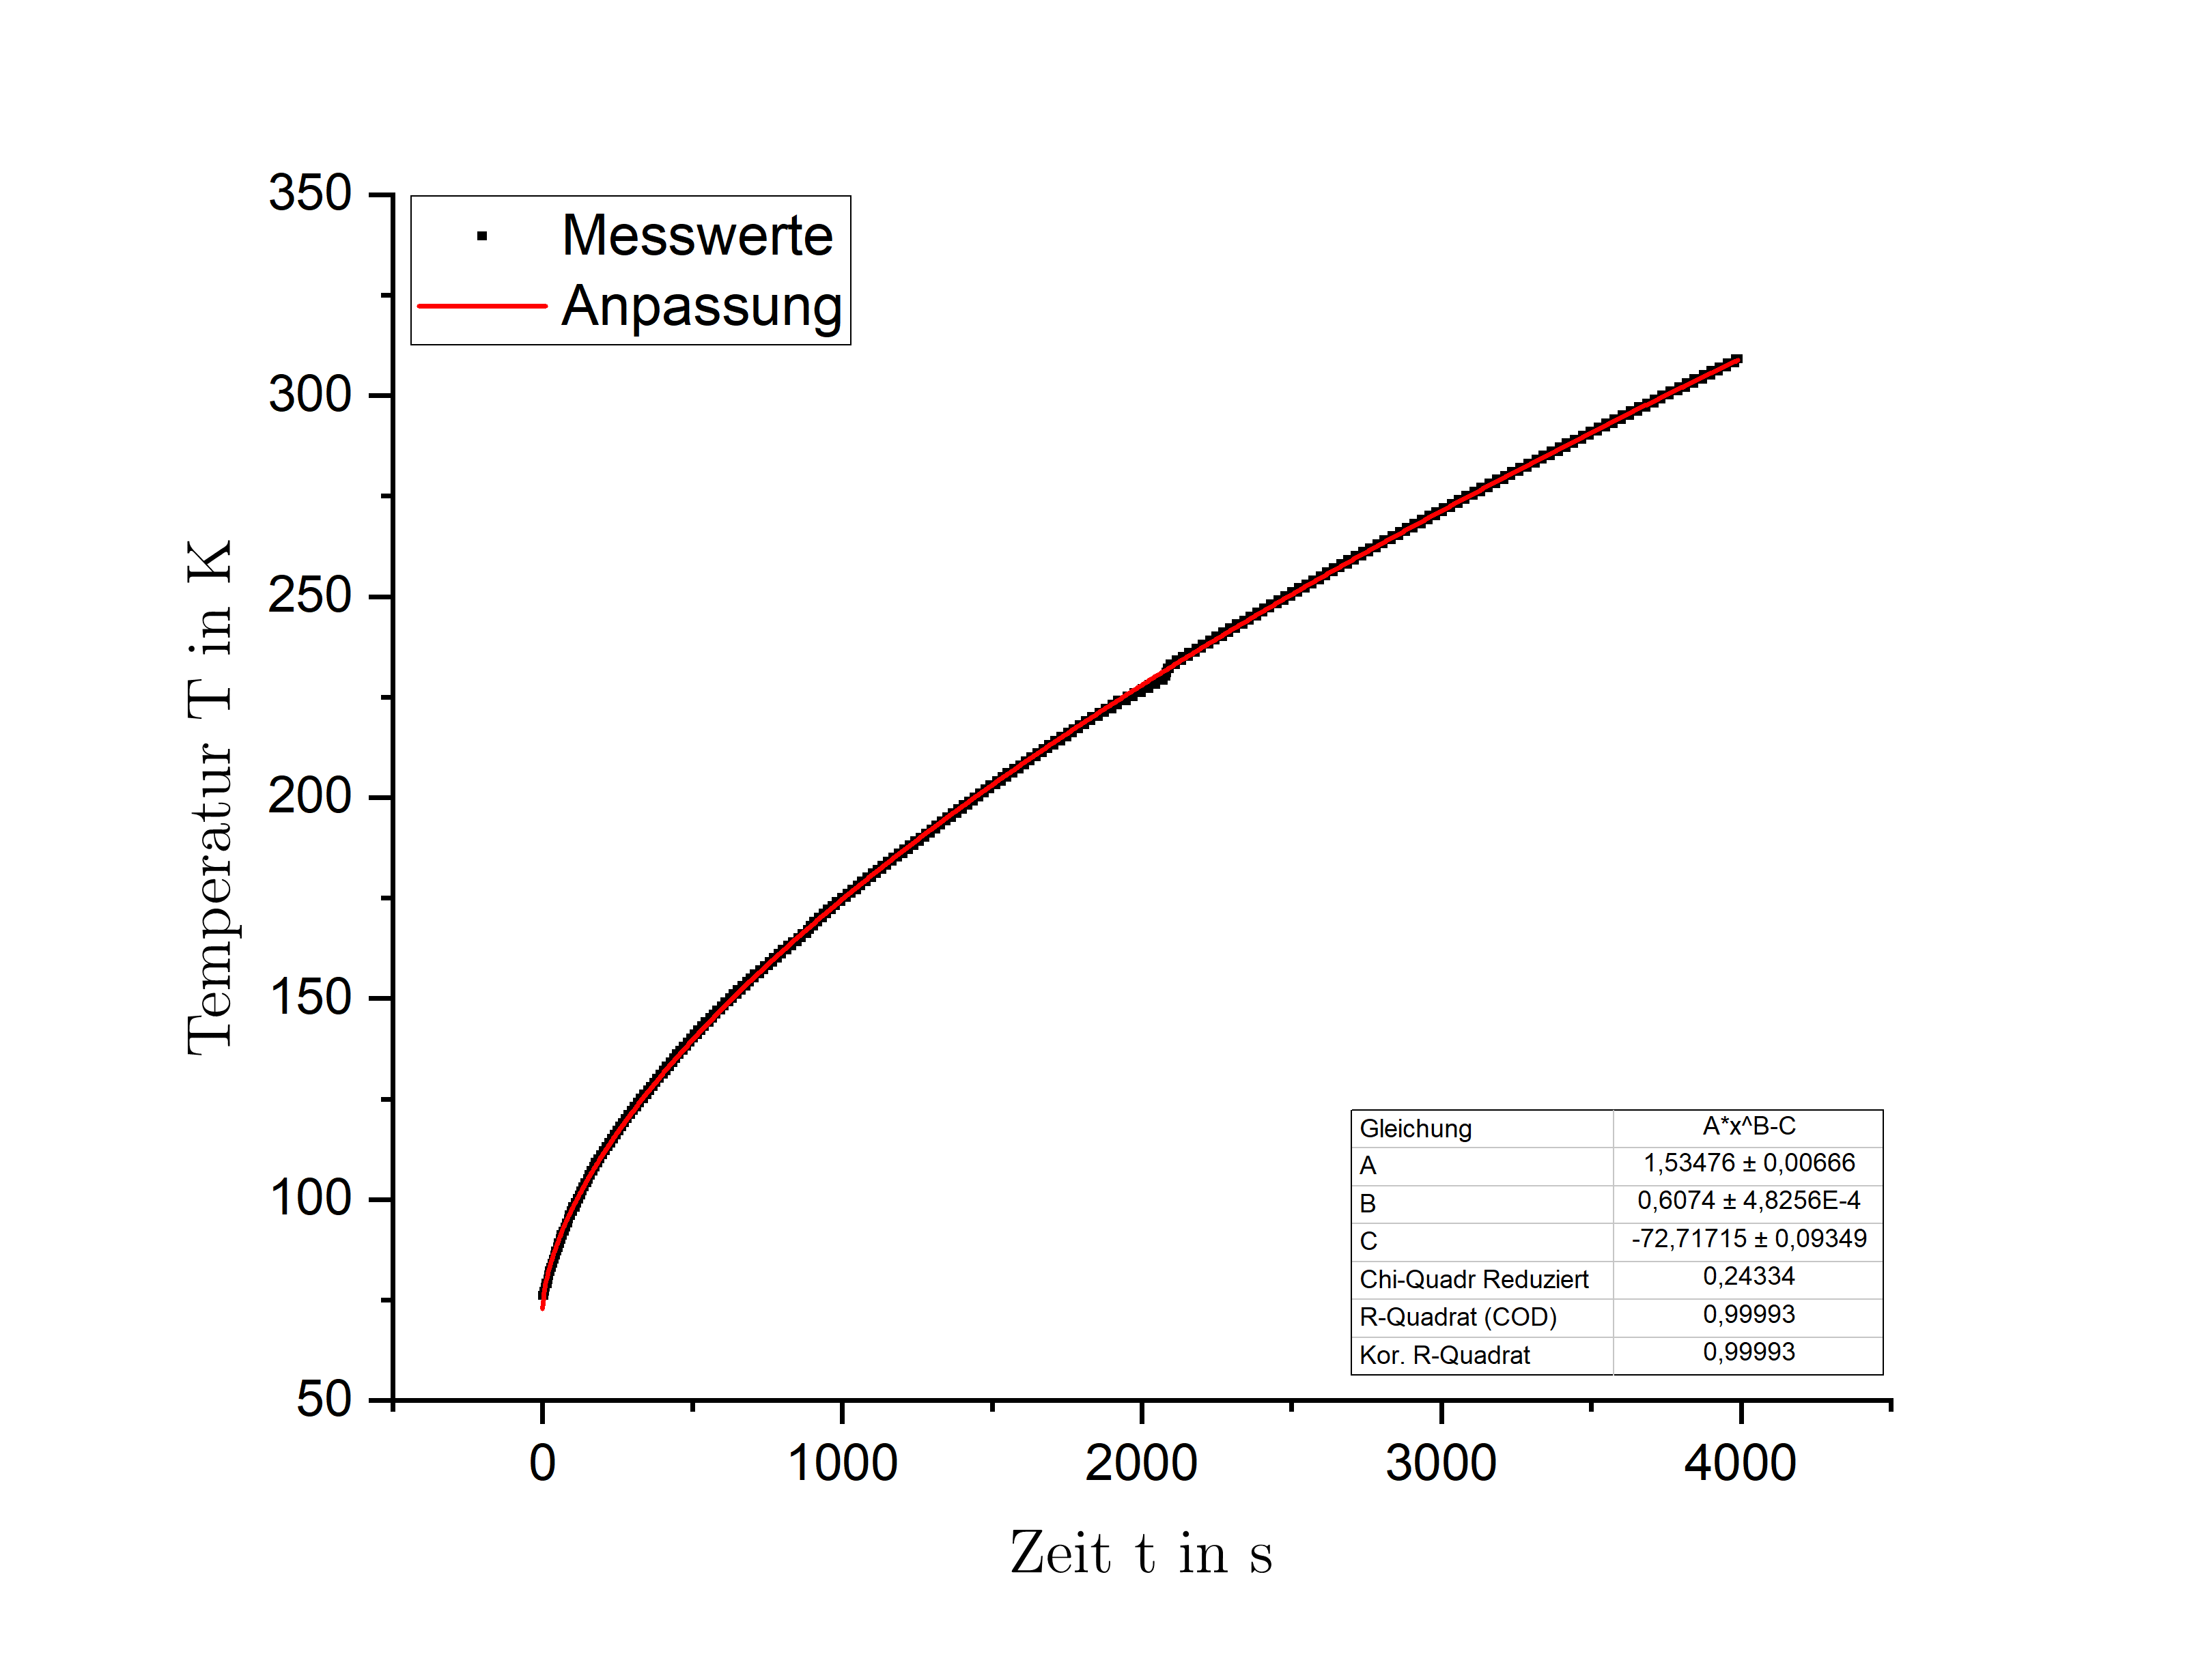
\includegraphics[scale=0.5]{fig/A2HeizinK.png}
    \caption{Temperaturkurve des beheizten Zylinders}
    \label{fig:heiz}
\end{figure}
\begin{figure}[H]
    \centering
    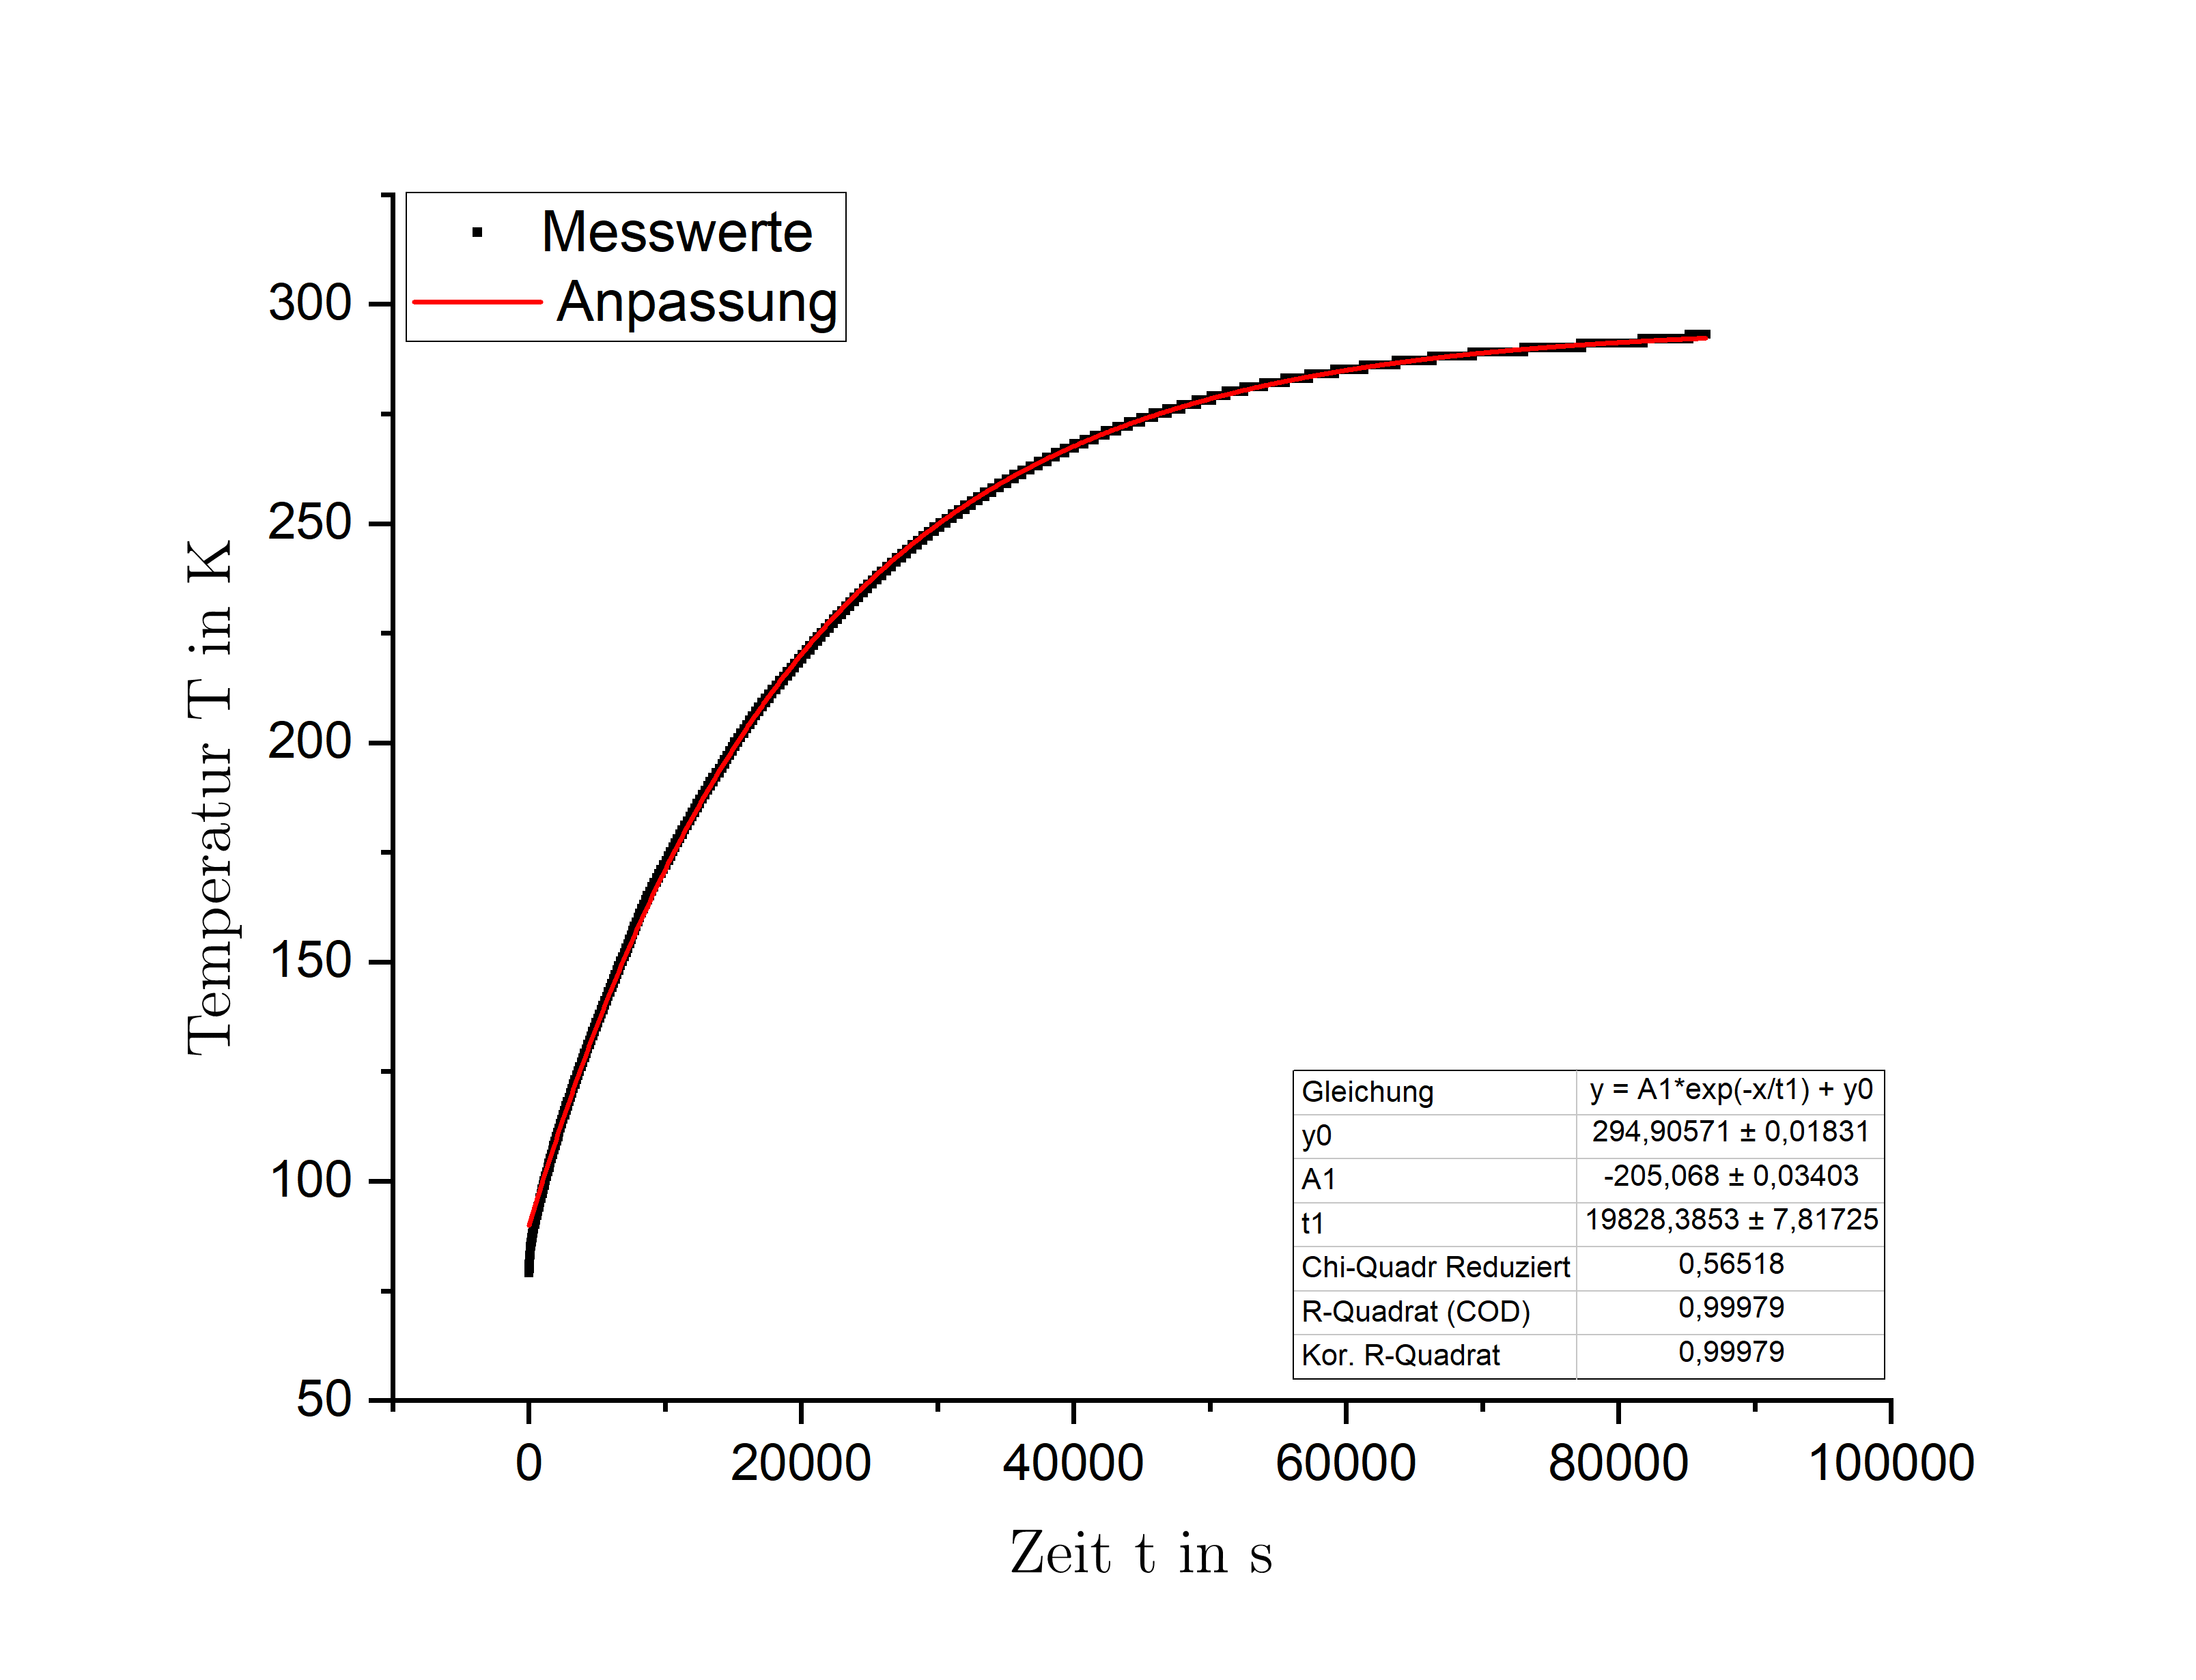
\includegraphics[scale=0.5]{fig/A2RauminK.png}
    \caption{Temperaturkurve des unbeheizten Zylinders}
    \label{fig:raum}
\end{figure}
Um aus diesen nun die Wärmekapazität bestimmen zu können, werden die Messdaten über einen annähernd passende Funktion gefittet, deren genau Form i.A. nicht von Relevanz ist. Einzig die Ableitung der gefitteten Funktion wird numerisch für eine Differentialgleichung benötigt, die explizite Form des Fits lässt sich unter umständlichem Lösen einer Differentialgleichung allerdings auch berechnen. Das Prinzip der Rechnung besteht darin, die Wärme des Systems $Q=c \cdot T$ und deren Änderungen zu betrachten, wobei bei beiden Messreihen Wärme von der Umgebung aufgenommen wird, allerdings nur bei der beheizten noch eine zusätzliche Heizleistung P hinzukommt. Dies lässt sich wie folgt ausdrücken ($c = c_\text{spez.} \cdot m$ und $\dot{c}(t) << 1$):
\begin{align}
    \frac{\d Q_\text{beheizt}}{\d t} &= \frac{\d (c\cdot T_H)}{\d t} \approx c\cdot \dot{T}_H(t) = P_\text{Heiz} + \alpha \cdot (T_\text{raum}-T_H(t)) \\
    \frac{\d Q_\text{unbeheizt}}{\d t} &= \frac{\d (c\cdot T_R)}{\d t} \approx c\cdot \dot{T}_R(t) = \alpha \cdot (T_\text{raum}-T_R(t))
\end{align}
Die Abhängigkeit von c von der Zeit wurde hier vernachlässigt, weil diese relativ klein ist, da sie lediglich die Abhängigkeit der Temperatur impliziert. Wird die Abhängigkeit der Wärmekapazität von der momentanen Temperatur nun berücksichtigt, und die momentane Temperatur somit als die neue Variable betrachtet, wobei die Ableitung allerdings als Zeitableitungen verbleiben, lassen sich $T_H$ und $T_K$ zusammenführen, da deren Zeitabhängigkeit nichtmehr relevant ist, und man kann Gl. 2.2 von Gl. 2.1 abziehen:
\begin{align}
    \frac{\d Q_\text{beheizt}}{\d t} - \frac{\d Q_\text{unbeheizt}}{\d t} &= P_\text{Heiz} = c(T) \cdot (\dot{T}_H(T)-\dot{T}_R(T)) \\
    \Rightarrow c_\text{spez.}(T) &= \frac{P_\text{Heiz}}{m} \cdot \frac{1}{\dot{T}_H(T)-\dot{T}_R(T)}
\end{align}
Die benötigten Kurven, berechnet aus Fits von Abbildungen \ref{fig:heiz} und \ref{fig:raum}, lassen sich in Abb. \ref{fig:t1} und \ref{fig:t2} finden. Die hieraus berechnete Wärmekapazität nach Gl. (2.4) lässt sich außerdem in Abb. \ref{fig:c} finden.
\begin{figure}[H]
    \centering
    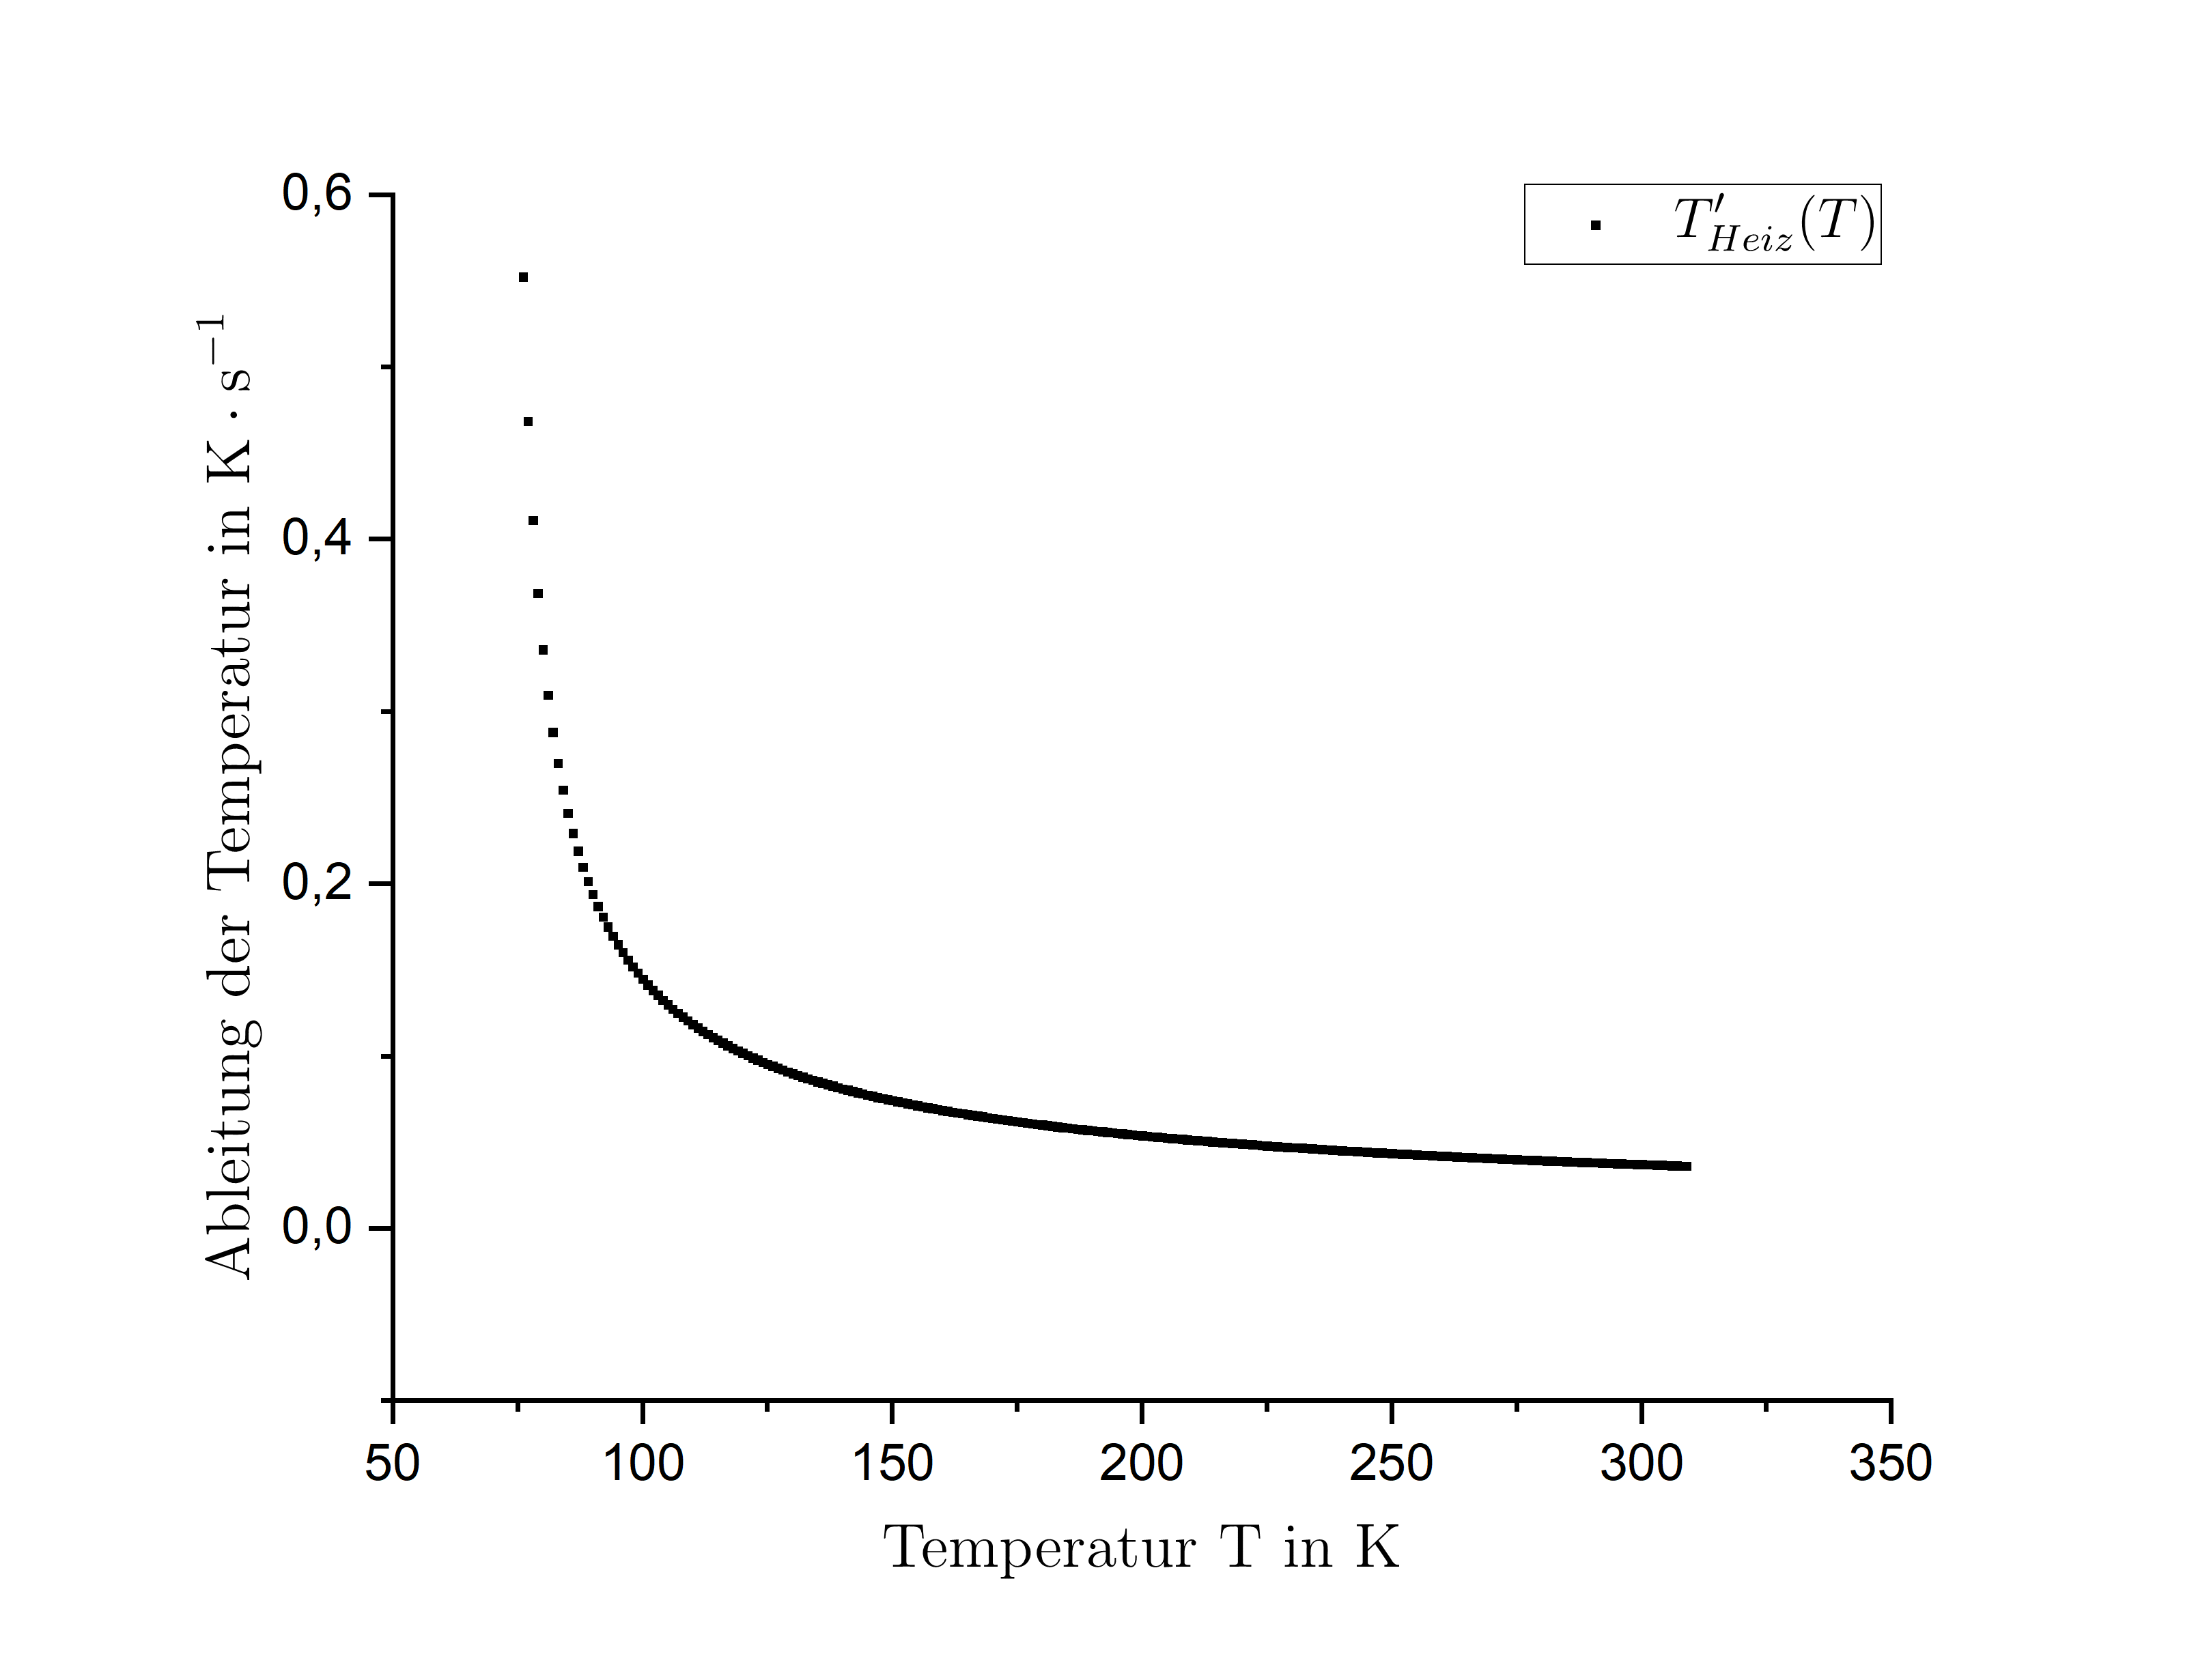
\includegraphics[scale=0.5]{fig/A2T'T.png}
    \caption{Abhängigkeit der Zeitableitung der Temperatur von sich selbst (beheizt)}
    \label{fig:t1}
\end{figure}
\begin{figure}[H]
    \centering
    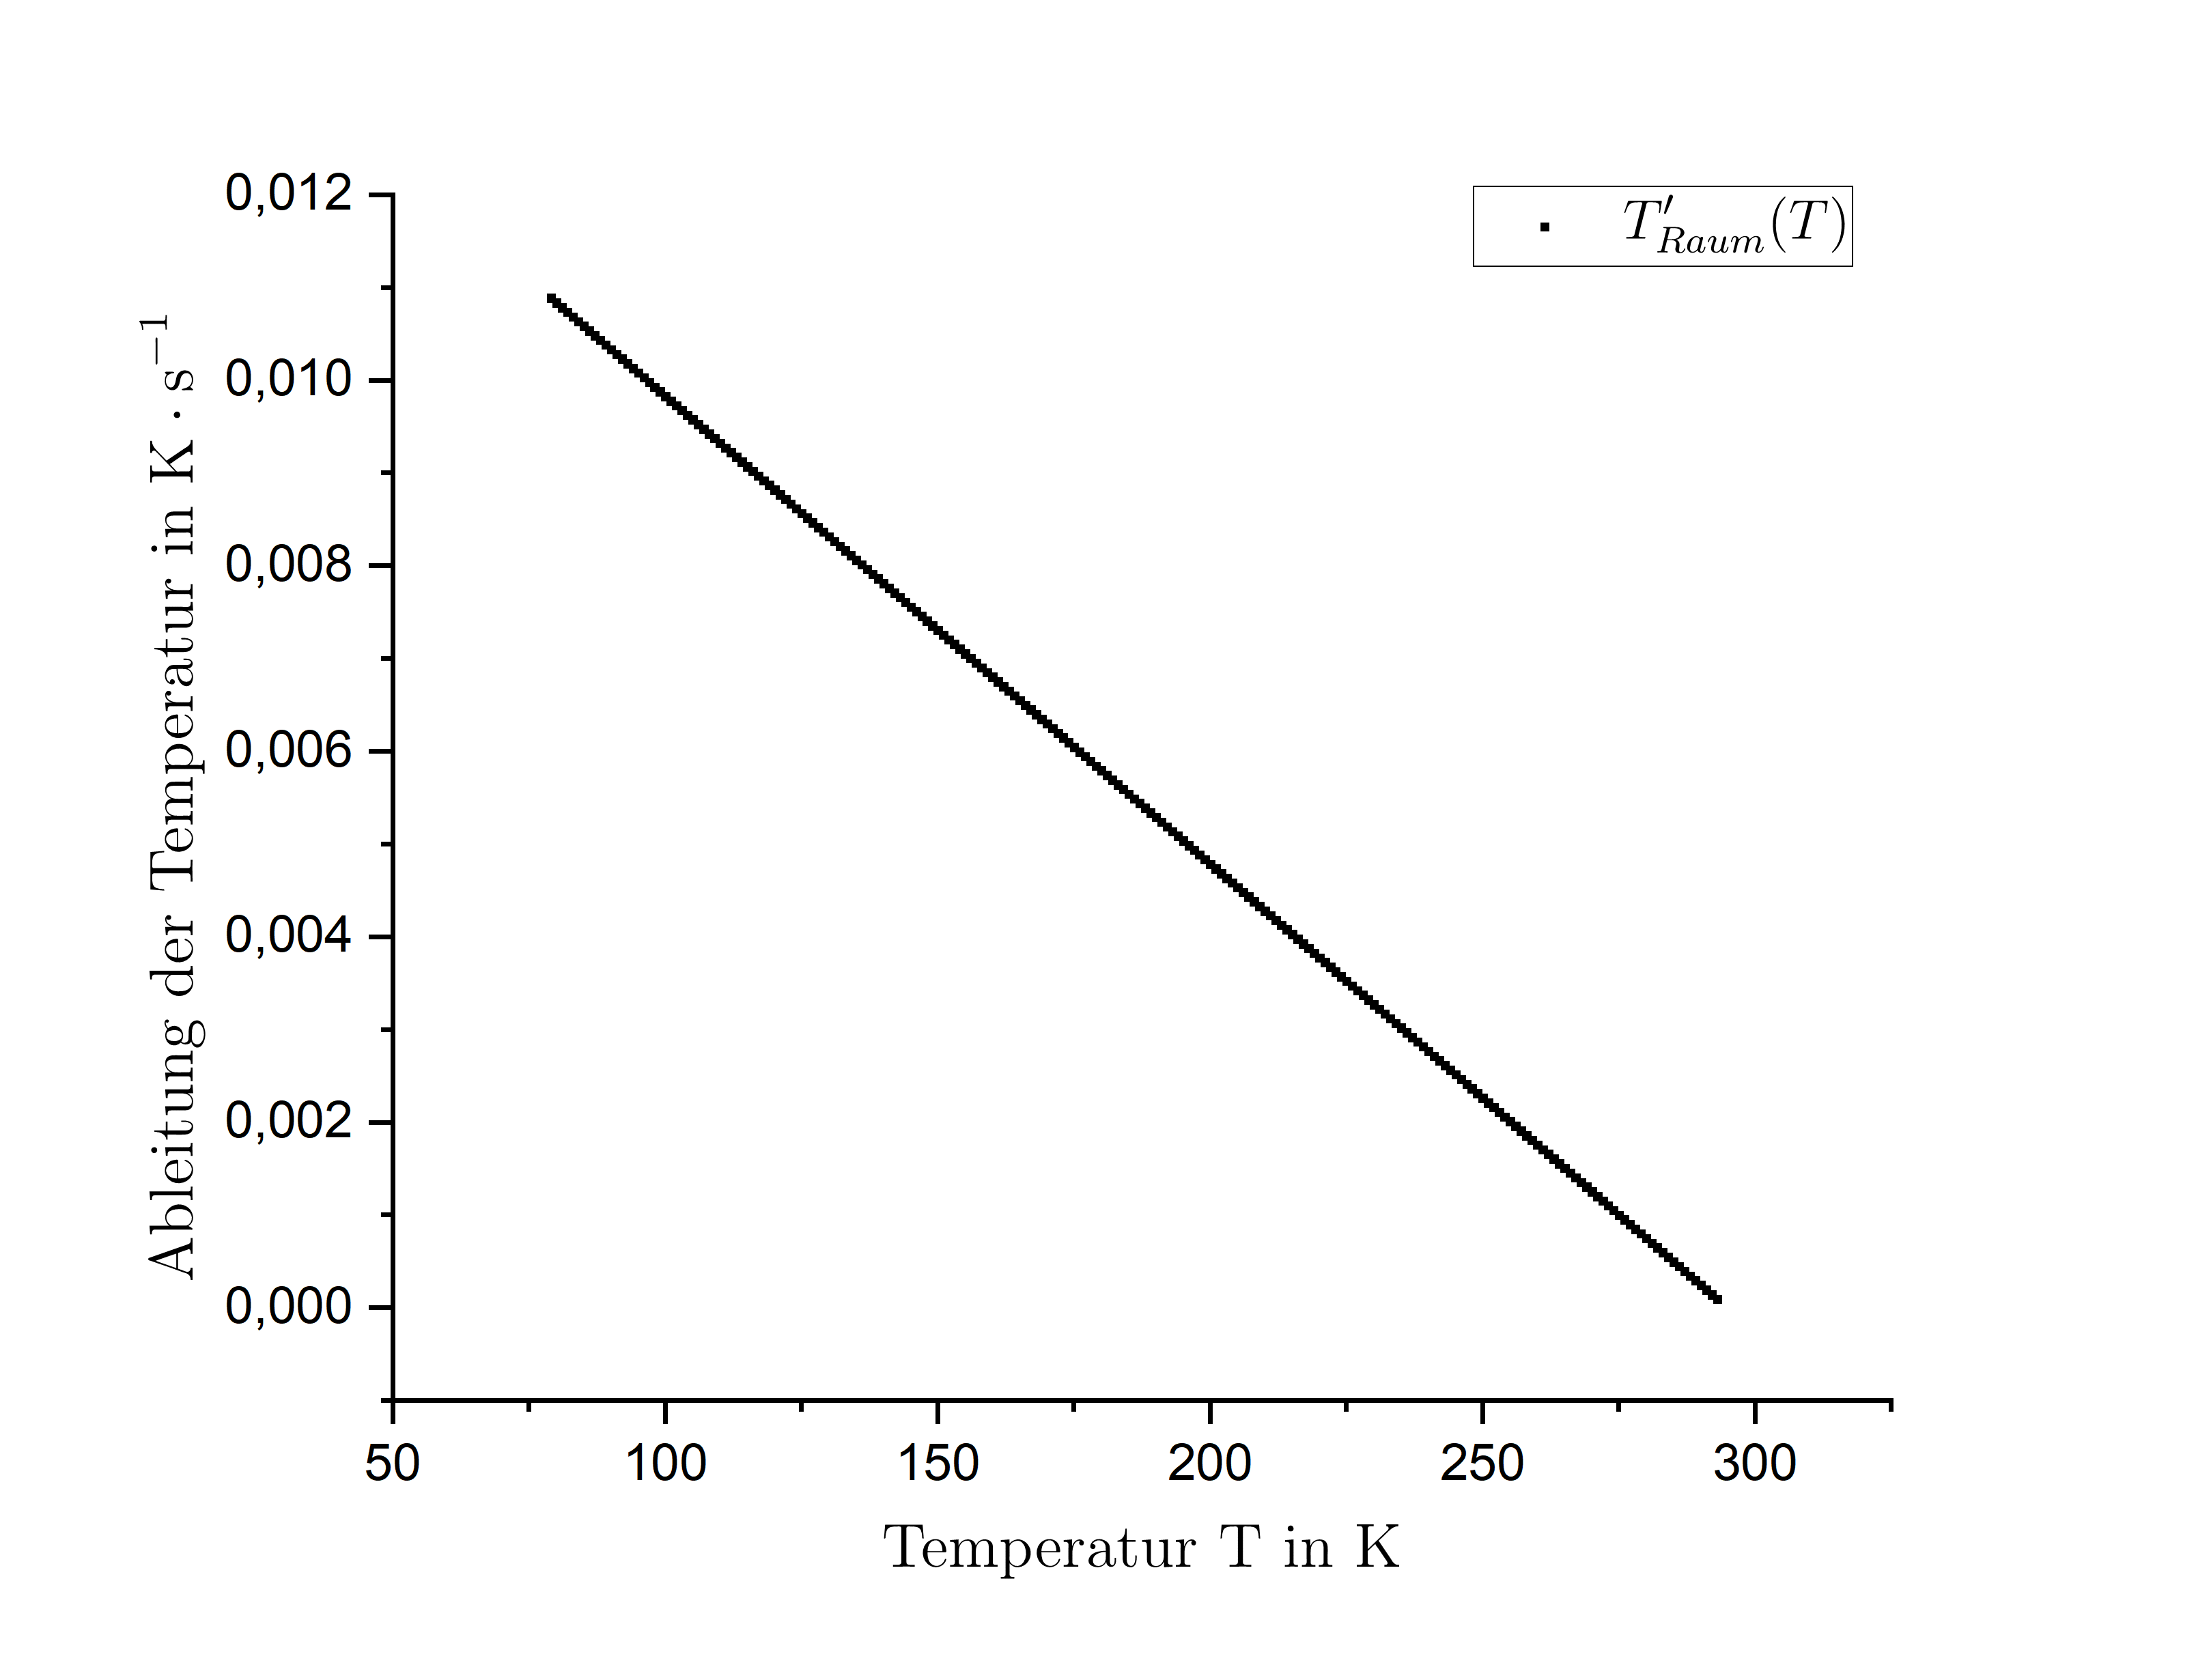
\includegraphics[scale=0.5]{fig/A2T'T1.png}
    \caption{Abhängigkeit der Zeitableitung der Temperatur von sich selbst \\ (unbeheizt)}
    \label{fig:t2}
\end{figure}
\begin{figure}[H]
    \centering
    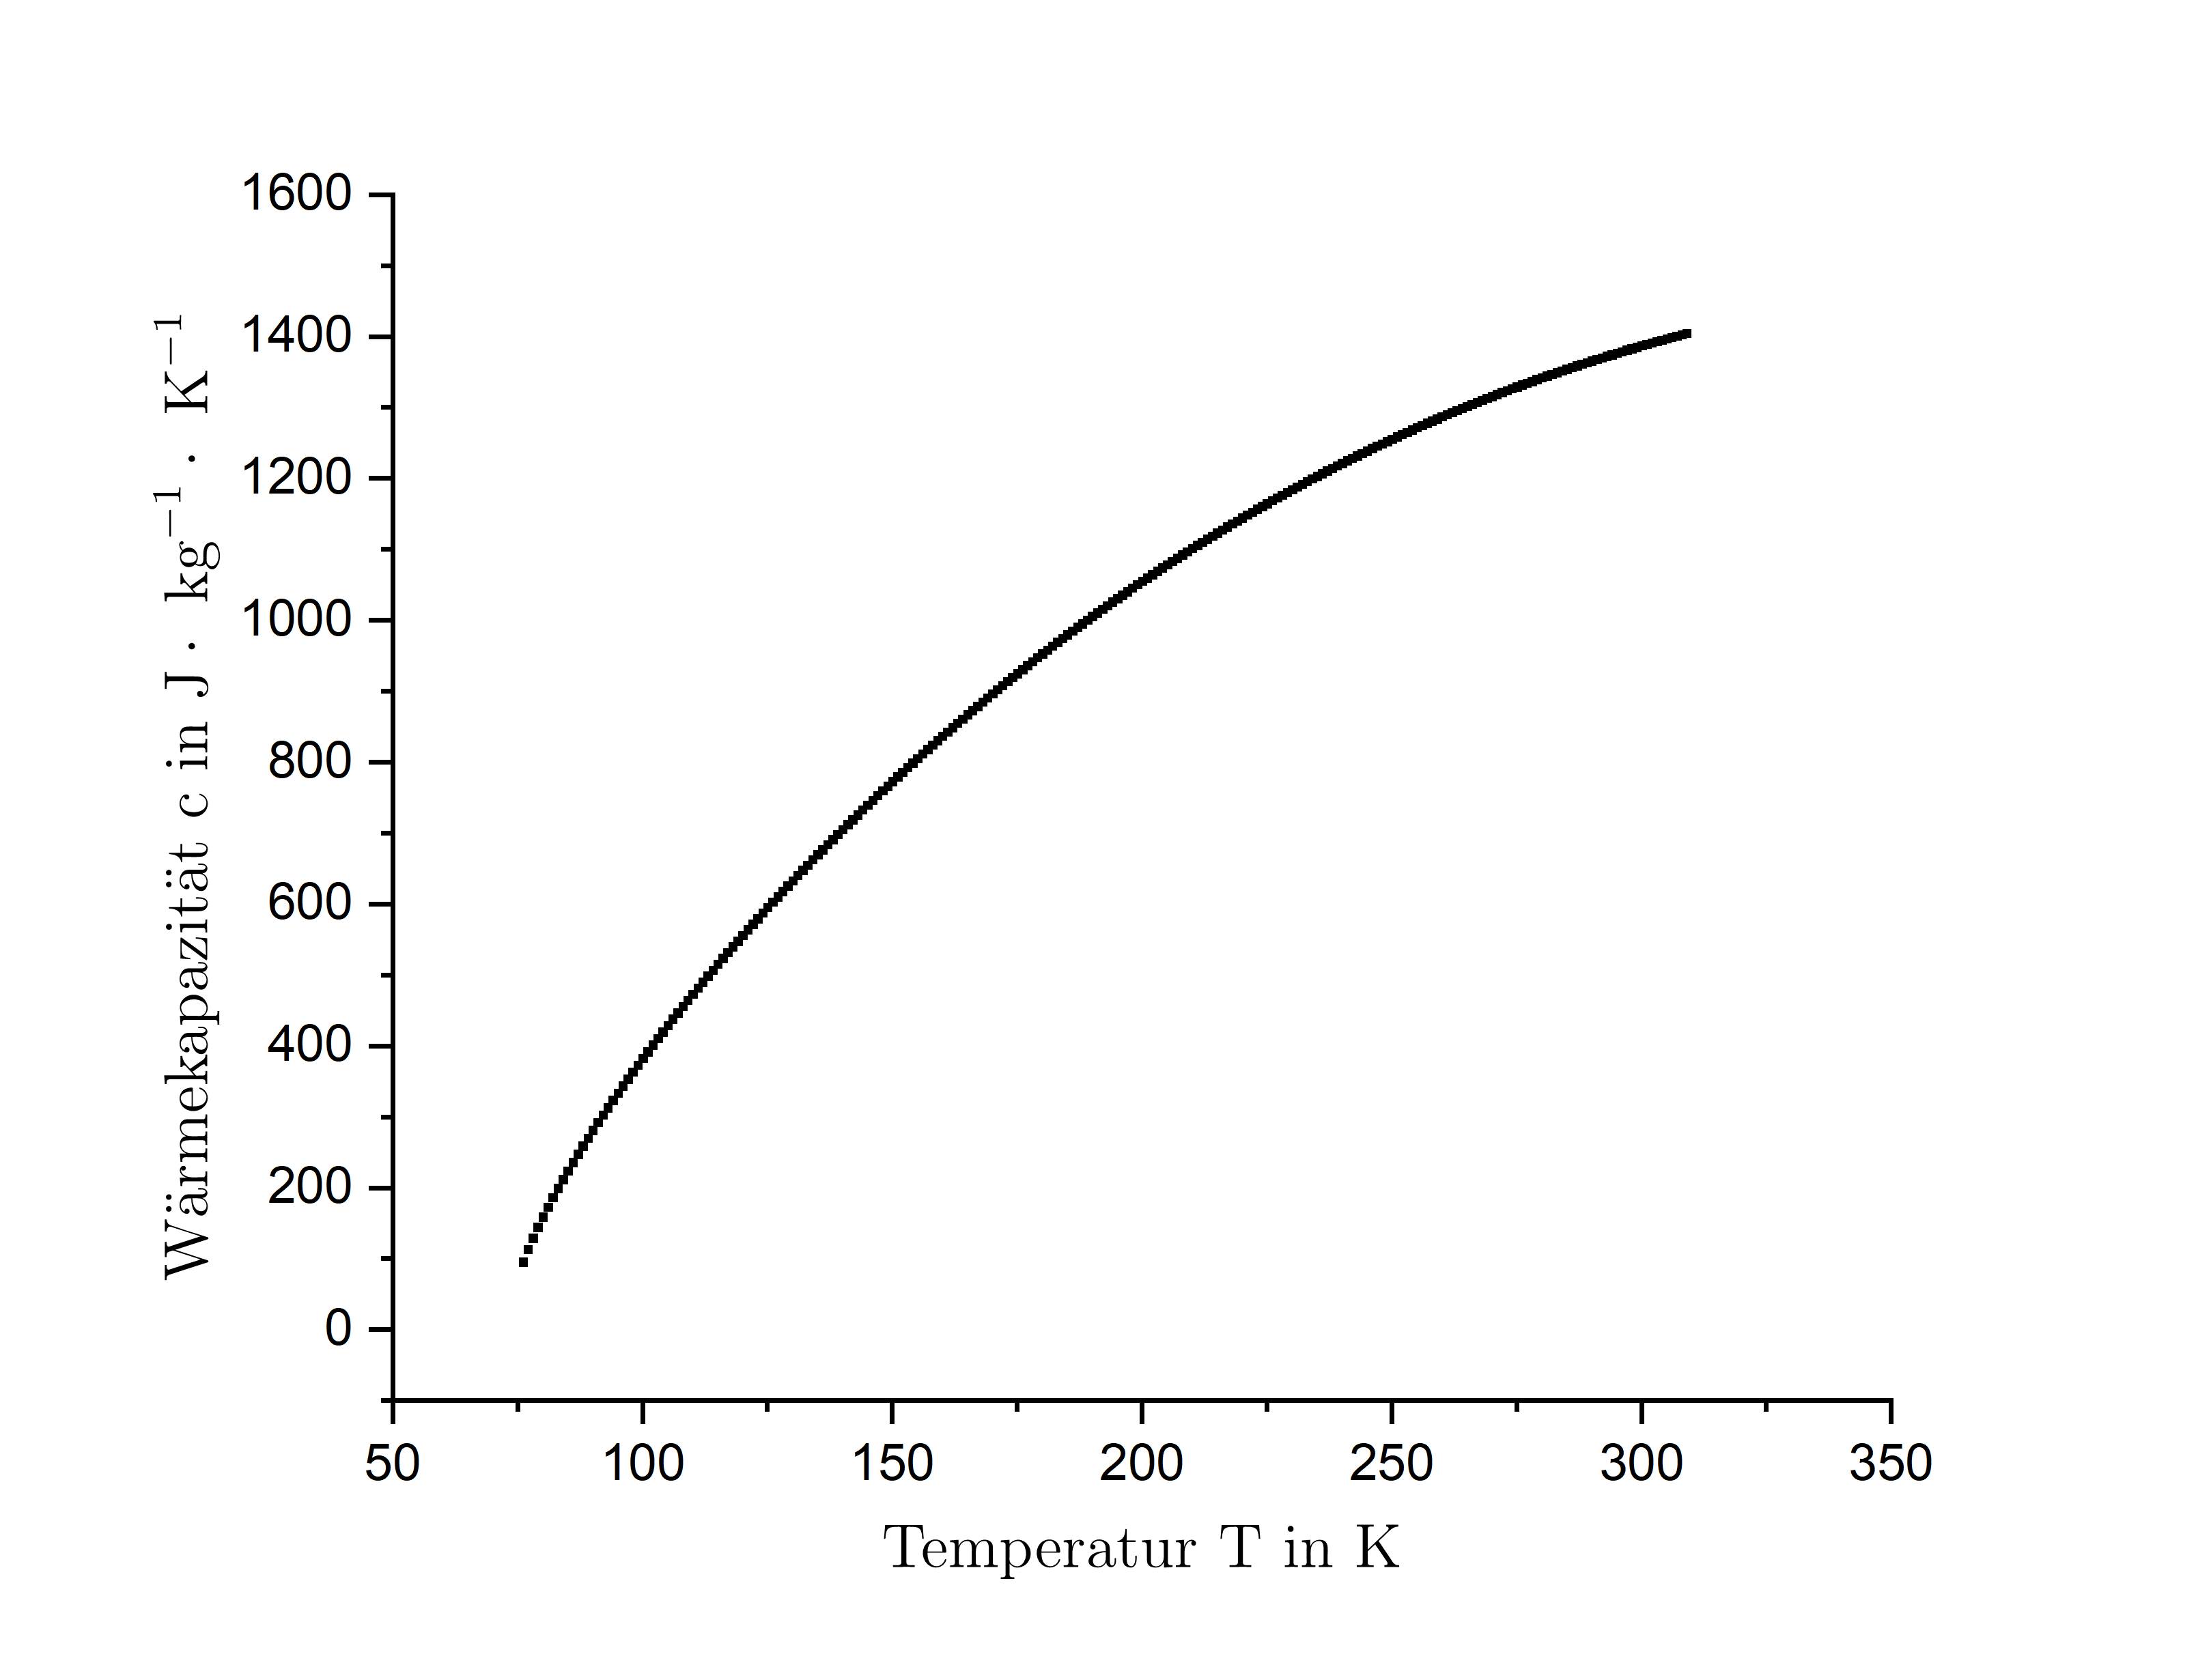
\includegraphics[scale=0.5]{fig/A2cT.png}
    \caption{Abhängigkeit der Wärmekapazität von der Temperatur}
    \label{fig:c}
\end{figure}
\clearpage
Wie zu sehen ist, ist die Wärmekapazität von der Temperatur vor allem bei tiefen Temperaturen stark von ihr abhängig, und bewegt sich für Temperaturen nahe der Raumtemperatur ($T \approx \SI{300}{K}$) in dem in Aufgabe 1 berechneten Bereich. Dies ist eigenartig, da die dort berechneten Werte als zu groß angenommen wurden, basierend auf Literaturwerten. Da die Anpassungskurven, wie in den Abbildungen \ref{fig:heiz} und \ref{fig:raum} zu sehen, den Messdaten relativ gut folgen, sollten die hieraus folgenden numerischen Fehler auch relativ klein sein. Weiterhin könnte sich die benutzte Anpassungsfunktion doch als relevant erweisen, allerdings würde diese lediglich Abb. \ref{fig:t2} beeinflussen, und dessen Werte für hohe Temperaturen liegen ohnehin schon im Bereich um 0. Demnach wird entweder die Heizleistung größer sein als erwartet, die Masse des Aluminiumzylinder kleiner sein als erwartet, oder die Zeitableitung der Temperatur der beheitzten Messreihe ist kleiner als erwartet. Dies deutet darauf hin, dass es Fremdfaktoren gab, welche eine zusätzliche Wärmekapazität ins System eingebracht haben, welche fehlerhaft in die des Aluminiums miteinberechnet wurden. Eine weitere Möglichkeit für die Abweichung lässt sich in der Referenzsonde finden, welche nach dem Experiment nicht nochmal nachgeprüft wurde. Falls das Eis während des Versuchs geschmolzen ist, würde demnach die Referenz langsam durch Umwelteinflüsse nach oben driften, was zu einer relativen zeitlichen Verkleinerung der gemessenen Spannungen führen würde. Dies ließe sich in aufgrund der Beheizung nur schwer an einem etwaigen Grenzwert o.ä. feststellen, es würde lediglich eine zeitliche Verzögerung der Kurve entstehen, welche nur schwer zu erkennen ist. Diese zeitliche Verzögerung würde allerdings zu einer Verkleinerung der zeitlichen Änderung der Temperatur nach der Zeit führen, wodurch auch die Wärmekapazität zwar für tiefe Temperaturen gut den Literaturwerten entsprechen, für hohe aber darüber liegen müsste.

\end{document}

